
\chapter{Week10}

\section{Wednesday}\index{week10_Tuesday_lecture}
\subsection{Preliminaries on Notations}
The notations in this course are slightly different from that in textbook or other sources. Let's make a justification, for example:
\begin{enumerate}
\item
Derivative:
\[
\begin{array}{lllllll}
\frac{\partial F}{\partial x_i},
&
F_{x_i},
&
F_i,
&
\partial_{x_i}F,
&
\partial_iF,
&
D_{x_i}F,
&
D_iF
\end{array}
\]
\item
Gradient $\&$ Jacobian Matrix:
\begin{definition}[Gradient]
For $f:\mathbb{R}^n\to\mathbb{R}$, its \emph{gradient} $\nabla f(\bm x)$ is a $n\times1$ \emph{column vector}:
\[
[\nabla f(\bm x)]_i=\frac{\partial f}{\partial x_i}(\bm x)
\]
its \emph{Jacobian} matrix $Df(\bm x)$ is a $n\times1$ \emph{row vector}:
\[
Df(\bm x)=\nabla\trans f(\bm x)
\]
\end{definition}
\begin{definition}[Jacobian matrix]
For $f:\mathbb{R}^n\to\mathbb{R}^m$, suppose $f=(f_1,f_2,\dots,f_m)$, then the $j$-th row of \emph{Jacobian matrix} of $f$ is just the transpose of $\nabla f_j(\bm x)$: 
\[
Df(\bm x)=\begin{pmatrix}
Df_1(\bm x)\\Df_2(\bm x)\\\vdots\\Df_m(\bm x)
\end{pmatrix}=\begin{pmatrix}
\nabla\trans f_1(\bm x)\\
\nabla\trans f_2(\bm x)\\
\vdots\\
\nabla\trans f_m(\bm x)\\
\end{pmatrix}
\]
\end{definition}
\end{enumerate}

This lecture will discuss some preliminaries and properties on multi-variate differentiation. Next lecture we will turn into implicit function theorem.

\subsection{Analysis on multi-variate differentiation}
First let's extend the chain rule to the multi-variate situation:
\begin{definition}[Composition]
Suppose $X\subseteq\mathbb{R}^n$ and $Y\in\mathbb{R}^m$.  The function $f$ maps $X$ into $Y$, and the function $g$ maps $Y$ into $\mathbb{R}^k$. If $f,g$ are differentiable at $\bm x=\bm x_0$, i.e., the Jacobian matrix $Df(x_0)\in\mathbb{R}^{m\times n},Dg(x_0)\in\mathbb{R}^{k\times m}$ is well-defined, then the mapping $g\circ f$ is also differentiable at $\bm x=\bm x_0$, with the derivative
\[
D(g\circ f)(\bm x_0)
=
Dg(f(\bm x_0))* Df(\bm x_0),
\]
or rewriting it into matrix form: ($\bm y_0:=f(\bm x_0)$)
\item
\begin{align*}
D(g\circ f)(\bm x_0):&=\begin{pmatrix}
\frac{\partial }{\partial x_1}(g_1\circ f)&\cdots&\frac{\partial }{\partial x_n}(g_1\circ f)\\
\vdots&\ddots&\vdots\\
\frac{\partial }{\partial x_1}(g_k\circ f)&\cdots&\frac{\partial }{\partial x_n}(g_k\circ f)
\end{pmatrix}_{k\times n}\\
&=
\begin{pmatrix}
\frac{\partial g_1}{\partial y_1}(\bm y_0)&\cdots&\frac{\partial g_1}{\partial y_m}(\bm y_0)\\
\vdots&\ddots&\vdots\\
\frac{\partial g_k}{\partial y_1}(\bm y_0)&\cdots&\frac{\partial g_k}{\partial y_m}(\bm y_0)
\end{pmatrix}_{k\times m}
\begin{pmatrix}
\frac{\partial f_1}{\partial x_1}(\bm x_0)&\cdots&\frac{\partial f_1}{\partial x_n}(\bm x_0)\\
\vdots&\ddots&\vdots\\
\frac{\partial f_m}{\partial x_1}(\bm x_0)&\cdots&\frac{\partial f_n}{\partial x_n}(\bm x_0)
\end{pmatrix}_{m\times n}
\end{align*}
\end{definition}
The proof is similar to the one-dimension case.


\begin{definition}[Directional Derivative]
Given a function $f:X(\subseteq\mathbb{R}^n)\mapsto\mathbb{R}^m$, for fixed $\bm x_0$ in $E$, suppose $\bm v\in\mathbb{R}^n$ is a unit vector, then the \emph{directional derivative} of $f$ at $\bm x=\bm x_0$ in the direction of $\bm v$ is given by:
\begin{equation}\label{Eq:10:1}
D_{\bm v}f(\bm x_0)=\lim_{t\to0}\frac{f(\bm x_0+t\bm v) - f(\bm x_0)}{t},
\end{equation}
where $t\in\mathbb{R}$.
\end{definition}
\begin{proposition}
The formula (\ref{Eq:10:1}) can be re-written as:
\begin{equation}
D_{\bm v}f(\bm x_0)=Df(\bm x_0)*\bm v,
\end{equation}
with the operator $*$ being the matrix multiplication.
\end{proposition}
\begin{proof}
For fixed $\bm x_0$, let $g(t)=f(\bm x_0+t\bm v)$ to be the one-argument scalar function, it follows that
\begin{align*}
\lim_{t\to0}\frac{f(\bm x_0+t\bm v) - f(\bm x_0)}{t}&=\lim_{t\to0}\frac{g(t) - g(0)}{t}\\
&=g'(0)\\
&=[Df(\bm x_0+t\bm v)*\bm v]_{t=0}\\
&=Df(\bm x_0)*\bm v
\end{align*}
\end{proof}
\begin{corollary}
Given the $n$-argument scalar function $f:\mathbb{R}^n\to\mathbb{R}$, the \emph{directional derivative} of $f$ at $\bm x=\bm x_0$ in the direction of $\bm v$ can be expressed as:
\[
D_{\bm v}f(\bm x_0)=\inp{\nabla f(\bm x_0)}{\bm v}.
\]
\end{corollary}
Thus we have defined the derivative for multi-variate function at any direction. Now we study in which direction does the function decrease/increase at the fastest rate.



\begin{example}
The gradient actually tells us how the function behaves locally. Given a simple function $f(x,y)=x^2+y^2$, its \emph{level curve} is given as follows:
\begin{figure}[H]
\centering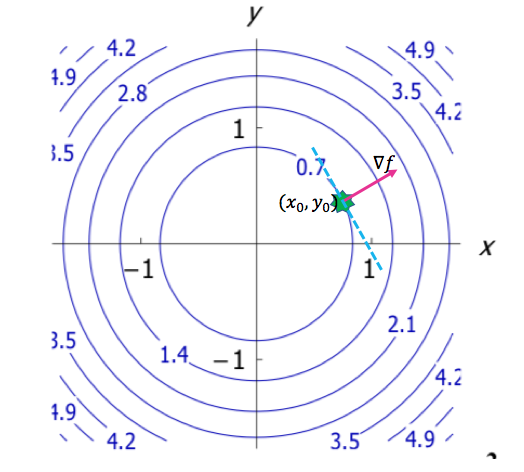
\includegraphics[width=8cm]{week10/f_10_2}
\caption{Contour plot for $f(x,y)=x^2+y^2$}
\end{figure}
where each contour refers to the set $\{(x,y)\mid f(x,y) = \mbox{constant C}\}$.

The gradient at $(x_0,y_0)$ is given by:
\[
\nabla f(x_0,y_0) = (2x_0,2y_0)\trans.
\]
The tangent plane at $x^2+y^2=C$ can be denoted as a vector:
\[
P=(-y,x)
\]
Since $\inp{\nabla f(x_0,y_0)}{P|_{(x_0,y_0)}}=0$, the gradient $\nabla f(x,y)$ is perpendicular to the level curves, with the direction pointing to where the function $f$ increases the fastest.
\end{example}
\begin{proposition}
For $f:\mathbb{R}^n\to\mathbb{R}$, the direction $\frac{\nabla f(\bm x)}{\|\nabla f(\bm x)\|}$ gives the direction at which the function increases the fastest; the direction $-\frac{\nabla f(\bm x)}{\|\nabla f(\bm x)\|}$ gives the direction at which the function decreases the fastest.
\end{proposition}
The proof is simply by applying the Cauchy-Schawz inequality.
\paragraph{Interpretation in one-dimension} For $n=1$, when $f'>0$, $f$ is increasing; when $f'<0$, $f$ is decreasing. Thus the sign of $f'$ tells us at which direction the function increases/decreases. 
\begin{proposition}[Algebra Rules for Gradients]
Given two functions $f:X(\subseteq\mathbb{R}^n)\mapsto\mathbb{R}$ and $g:X(\subseteq\mathbb{R}^n)\mapsto\mathbb{R}$, if both $f,g$ are differentiable, the product and division are also differentiable. In particular,
\begin{align*}
\nabla (gf)&=g(\nabla f)+f(\nabla g)\\
\nabla(f/g)&=\frac{g\nabla f - f\nabla g}{g^2}
\end{align*}
\end{proposition}


\begin{theorem}[Mean-Value Theorem]
Let $f:X\subseteq\mathbb{R}^m\mapsto\mathbb{R}^n$ be differentiable in $X$, and $f=(f_1,f_2,\dots,f_n)$. If $\bm x$ and $\bm y$ are two points in $X$ such that the line segment $L$ connecting $\bm x$ and $\bm y$ lies completely in $X$, then $\exists \bm c_1,\bm c_2,\dots,\bm c_n \in L$ such that
\[
f_j(\bm x)-f_j(\bm y)=\inp{\nabla f_j(c_j)}{\bm x-\bm y},j=1,2,\dots,n
\]
or equivalently,
\[
f(\bm x)-f(\bm y)=Df(\bm c)*(\bm x-\bm y).
\]
\end{theorem}
\begin{proof}
For fixed $\bm x,\bm y$, define a one-argument scalar function
\[
\begin{array}{ll}
\phi(t)=f(\bm x+t(\bm y-\bm x)),
&
0\le t\le 1
\end{array}
\]
Applying MVT for one-variable, we derive
\[
\phi(1)-\phi(0)=\phi'(t)(1-0)
\]
Or equivalently,
\[
f(\bm y) - f(\bm x)=Df(\underbrace{\bm x+t(\bm y-\bm x)}_{\bm c})*(\bm y-\bm x)
=\inp{\nabla f(\bm c)}{\bm y-\bm x}
\]
\end{proof}
When can we change the order of differentiation?
\begin{example}
\[
f(x,y)=\left\{
\begin{aligned}
xy\frac{x^2-y^2}{x^2+y^2},&\quad (x,y)\ne(0,0)\\
0,&\quad x=y=0
\end{aligned}
\right.
\]
After messy computation, we find
\[
\frac{\partial^2f}{\partial x\partial y}(0,0)=
\frac{\partial }{\partial x}\left[\frac{\partial f}{\partial y}\right](0,0)=1\ne-1=\frac{\partial^2f}{\partial y\partial x}(0,0),
\]
i.e., we cannot change the order of differentiation without a careful scrutiny. 
\end{example}
\begin{theorem}
If $f:E(\subseteq\mathbb{R}^n)\mapsto\mathbb{R}^m$ has partial derivatives $\frac{\partial^2 f}{\partial x_i\partial x_j}$ and $\frac{\partial^2 f}{\partial x_j\partial x_i}$, then
\[
\frac{\partial^2 f}{\partial x_i\partial x_j}=\frac{\partial^2 f}{\partial x_j\partial x_i}
\]
at every point $x\in E$ where both partial derivatives are continuous.
\end{theorem}
\begin{corollary}
Generalizing it into higher orders
\end{corollary}
\begin{proof}
w.l.o.g., assume $i=1,j=2$. Define
\begin{align*}
F(h_1,h_2) &= f(x_1+h_1,x_2+h_2) - f(x_1+h_1,x_2) - f(x_1,x_2+h_2)+f(x_1,x_2)
\end{align*}
where the rectangle with vertices $(x_1,x_2),(x_1+h_1,x_2),(x_1,x_2+h_2),(x_1+h_1,x_2+h_2)$ are in $E$. We Define
\[
\phi(t)=f(x_1+th_1,x_2+h_2) - f(x_1+th_1,x_2),
\]
then
\[
F(h_1,h_2) = \phi(1) - \phi(0)=\phi'(\theta_1)
\]
Note that
\[
\phi'(t) = \frac{\partial f}{\partial x_1}(x_1+th_1,x_2+h_2)h_1 - \frac{\partial f}{\partial x_1}(x_1+th_1,x_2)h_1
\]
which follows that
\begin{align*}
F(h_1,h_2)=\phi'(\theta_1)
&=
\left[\frac{\partial f}{\partial x_1}(x_1+\theta_1h_1,x_2+h_2)h_1 - \frac{\partial f}{\partial x_1}(x_1+\theta_1h_1,x_2)\right]h_1\\
&=\frac{\partial }{\partial x_2}\frac{\partial f}{\partial x_1}(x_1+\theta_1h_1,x_2+\theta_2h_2)h_2h_1\\
&=\frac{\partial^2f}{\partial x_2\partial x_1}(x_1+\theta_1h_1,x_2+\theta_2h_2)h_1h_2
\end{align*}
Applying the same trick, we derive 
\[
\frac{\partial^2f}{\partial x_2\partial x_1}(x_1+\theta_1h_1,x_2+\theta_2h_2)h_1h_2=F(h_1,h_2)
=
\frac{\partial^2f}{\partial x_1\partial x_2}(x_1+\theta_3h_1,x_2+\theta_4h_2)h_1h_2
\]
or
\[
\frac{\partial^2f}{\partial x_2\partial x_1}(x_1+\theta_1h_1,x_2+\theta_2h_2)
=
\frac{\partial^2f}{\partial x_1\partial x_2}(x_1+\theta_3h_1,x_2+\theta_4h_2)
\]
for some $\theta_1,\theta_2,\theta_3,\theta_4$ between $(0,1)$. Taking $h_1,h_2\to0$, we conclude that
\[
\frac{\partial^2f}{\partial x_2\partial x_1}(x_1,x_2) = \frac{\partial^2f}{\partial x_1\partial x_2}(x_1,x_2)
\]


\end{proof}

